\documentclass[11pt]{article}
\usepackage[margin=1.1in]{geometry}
\usepackage{amsmath,amssymb}
\usepackage{booktabs}
\usepackage{array}
\usepackage{tabularx}
\usepackage[protrusion=true,expansion=false]{microtype}
\usepackage{xcolor}
\usepackage{enumitem}
\usepackage{titlesec}
\usepackage{tikz}
\usepackage{float}
\usetikzlibrary{arrows.meta,positioning,fit,calc,decorations.pathreplacing,shapes.geometric}
\usepackage{listings}
\usepackage{hyperref}
\hypersetup{colorlinks=true, linkcolor=blue!60!black, urlcolor=blue!60!black, citecolor=blue!60!black}
\usepackage[skip=0.6\baselineskip, indent=0pt]{parskip}

\titleformat{\section}{\large\bfseries}{\thesection.}{0.7em}{}
\titleformat{\subsection}{\normalsize\bfseries}{\thesubsection.}{0.6em}{}
\newcolumntype{L}{>{\raggedright\arraybackslash}X}

\lstdefinestyle{code}{
  basicstyle=\ttfamily\small,
  columns=fullflexible,
  keepspaces=true,
  breaklines=true,
  frame=single,
  framerule=0.3pt,
  xleftmargin=1em,
}

\definecolor{alice}{RGB}{230,240,255}
\definecolor{fixed}{RGB}{255,243,224}
\definecolor{chain}{RGB}{232,245,233}

\newenvironment{keypoint}{\begin{center}\begin{tabular}{|p{0.9\linewidth}|}\hline\rule{0pt}{2.6ex}}{\\\hline\end{tabular}\end{center}}

\title{\textbf{From a Rust program to one step on Bitcoin}\\How a withdrawal is proved, wrapped and disputed\\in LN-GAP 2.5}
\author{waxwing}
\date{October 2026 \\ \medskip An explainer for engineers with a basic familiarity with zero-knowledge proofs.\\Figures measured on the proof of concept (branch \texttt{v25-seal}).}

\begin{document}
\maketitle

\begin{abstract}
A withdrawal from the LN-GAP 2.5 sessions layer is a claim that a
program, run on some input, produced some output. Bitcoin cannot run
programs, so the claim travels through four machines: RISC Zero proves
the program's execution with a STARK; RISC Zero and gnark compress that
STARK into a 128-byte Groth16 proof; a fixed RISC-V program, BitVMX's
Groth16 verifier, checks that proof in about 478 million steps; and if
the two parties disagree about that check, they bisect its execution
off-chain until a single RISC-V instruction is left, which Bitcoin
Script can check. This note walks through each stage: what goes in, what
comes out, why the stage exists, where it runs and what it costs. It
ends with who does what in a normal withdrawal and in a dispute, and a
glossary.
\end{abstract}

\tableofcontents

\section{The problem, and the shape of the answer}
\label{sec:problem}

Alice has a channel with a hub. Her session contract holds bitcoin that
she may withdraw if she proves she returned the hub's tokens on a layer
2 (the L2). Normally the hub checks her proof itself and pays her in the
channel; nothing touches Bitcoin. But if the hub refuses, the claim must
be settled by Bitcoin, and Bitcoin's Script can do only small things: it
has no loops, a stack of 1,000 items and practical transaction sizes of
tens of kilobytes. It cannot verify a modern proof directly, let alone
re-run a program.

The answer combines two ideas.
\begin{enumerate}[leftmargin=1.5em]
\item \emph{Succinct proofs.} Instead of the program's whole execution,
  Alice shows a short proof that the execution happened and produced a
  given output. Checking the proof is far cheaper than re-running the
  program, and the proof is the same size whatever the program.
\item \emph{Optimistic bisection.} Even checking the proof is too much
  for Script (hundreds of millions of steps). But checking it is itself
  a deterministic program. If Alice and the hub disagree about its
  result, they can binary-search its execution for the first step on
  which they disagree. Bitcoin then only has to check that one step.
\end{enumerate}

\begin{figure}[H]
\centering
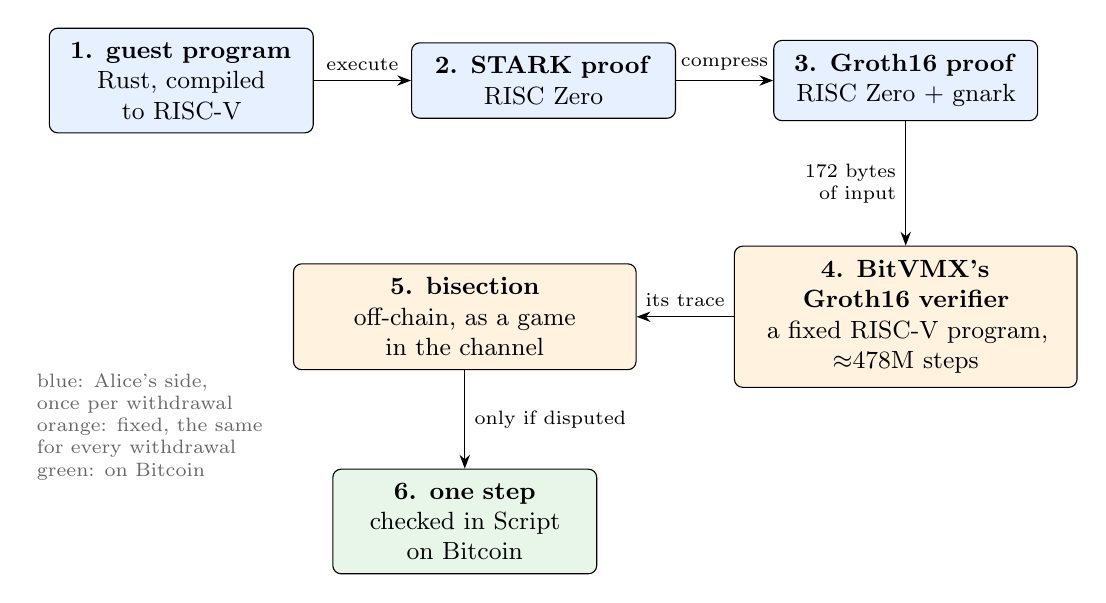
\begin{tikzpicture}[
  font=\small,
  box/.style={draw, rounded corners=3pt, align=center, inner sep=5pt, text width=#1},
  box/.default=30mm,
  >={Stealth[length=5pt]},
]
\node[box, fill=alice] (g) at (0,0) {\textbf{1. guest program}\\Rust, compiled to RISC-V};
\node[box, fill=alice] (s) at (4.6,0) {\textbf{2. STARK proof}\\RISC Zero};
\node[box, fill=alice] (w) at (9.2,0) {\textbf{3. Groth16 proof}\\RISC Zero + gnark};
\node[box=40mm, fill=fixed] (v) at (9.2,-3.0) {\textbf{4. BitVMX's Groth16 verifier}\\a fixed RISC-V program,\\$\approx$478M steps};
\node[box=40mm, fill=fixed] (b) at (3.6,-3.0) {\textbf{5. bisection}\\off-chain, as a game\\in the channel};
\node[box, fill=chain] (o) at (3.6,-5.6) {\textbf{6. one step}\\checked in Script\\on Bitcoin};
\draw[->] (g) -- node[above, font=\scriptsize] {execute} (s);
\draw[->] (s) -- node[above, font=\scriptsize] {compress} (w);
\draw[->] (w) -- node[left, font=\scriptsize, align=right] {172 bytes\\of input} (v);
\draw[->] (v) -- node[above, font=\scriptsize] {its trace} (b);
\draw[->] (b) -- node[right, font=\scriptsize] {only if disputed} (o);
\node[font=\scriptsize, text=black!60, align=left] at (-0.4,-4.4) {blue: Alice's side,\\once per withdrawal\\orange: fixed, the same\\for every withdrawal\\green: on Bitcoin};
\end{tikzpicture}
\caption{The pipeline. Stages 1--3 make a proof; stage 4 is the one
program anyone ever disputes; stages 5--6 happen only if the hub
disagrees with Alice about the result of stage 4.}
\label{fig:pipeline}
\end{figure}

\begin{keypoint}
There are \textbf{two different RISC-V programs} in this picture, run by
\textbf{two different machines}. Our statement (the guest) runs only in
RISC Zero's zkVM, on Alice's computer. BitVMX never sees it. BitVMX's
emulator runs only the Groth16 verifier, and it is the verifier's
execution that is bisected. The verifier is the same program for every
withdrawal and every statement.
\end{keypoint}

\section{Background: proofs, STARKs and SNARKs}
\label{sec:background}

\subsection{What a proof gives you}

A proof system lets a \emph{prover} convince a \emph{verifier} that a
\emph{statement} is true. For us the statement is always of one form:
\begin{center}
``program $P$, run on some input $w$, terminates and outputs $J$.''
\end{center}
The output $J$ is public (it is called the \emph{journal}); the input
$w$ is the prover's \emph{witness} and may stay private. A proof system
for such statements offers:
\begin{itemize}[leftmargin=1.5em]
\item \emph{Soundness:} if the statement is false, no prover can make
  the verifier accept, except with negligible probability.
\item \emph{Succinctness:} the proof is small and fast to check, much
  smaller and faster than re-running $P$.
\item \emph{Zero knowledge} (optional): the proof reveals nothing about
  $w$ beyond what $J$ says. This is what makes private payments
  possible; for the withdrawal itself we only need the first two.
\end{itemize}

Under the hood, a proof system turns the execution into a large set of
polynomial equations over a finite field (an \emph{arithmetisation}) and
proves that the equations hold without sending them all. Two families of
systems matter here, and they make opposite trade-offs.

\subsection{STARKs and SNARKs}

\begin{center}
\small
\begin{tabularx}{\linewidth}{@{}p{30mm}LL@{}}
\toprule
& STARK (as in RISC Zero) & Groth16 (a pairing-based SNARK) \\
\midrule
statement size & any program, any length (split into segments) & one fixed circuit \\
setup & transparent: no secrets & a trusted setup per circuit (a ceremony) \\
cryptography & hashes only (here Poseidon2 over the BabyBear field) & elliptic-curve pairings (here the BN254 curve) \\
proof size & hundreds of kilobytes & 3 curve points: 256 bytes, 128 compressed \\
verifier cost & many hash computations & 3 pairings and a few curve operations \\
prover cost & fast & slow, needs a lot of memory \\
\bottomrule
\end{tabularx}
\end{center}

The pipeline uses each for what it is good at. RISC Zero's STARKs prove
an arbitrary program cheaply. A Groth16 proof is what you want to hand
to a constrained verifier: small, with a fixed verification procedure.
So the STARK is proved first, and then a fixed Groth16 circuit proves
the single statement ``this STARK verifies''. Because that circuit is
the same for every program, one trusted setup serves everyone; RISC
Zero ran a public ceremony for it.

\paragraph{Fields.} Each system computes in its own finite field.
RISC Zero's STARK works modulo the 31-bit prime $p = 15 \cdot 2^{27} + 1$
(``BabyBear''), which suits fast hardware arithmetic. Groth16 over BN254
works modulo a 254-bit prime. Checking a BabyBear hash inside a BN254
circuit is very expensive, and this mismatch is the reason for an extra
step in Section~\ref{sec:wrap}.

\section{Stage 1: the guest program}
\label{sec:guest}

The statement is an ordinary Rust program, called the \emph{guest},
compiled for RISC Zero's zkVM: a 32-bit RISC-V machine (the RV32IM
instruction set: integer arithmetic, multiplication, division). It reads
private input from the host and writes public output to the journal.
The placeholder guest of the proof of concept:

\begin{lstlisting}[style=code]
use risc0_zkvm::guest::env;

fn main() {
    let (b, c): (u32, u32) = env::read();   // private input
    let mut journal = [0u8; 8];
    journal[..4].copy_from_slice(&b.to_le_bytes());
    journal[4..].copy_from_slice(&c.to_le_bytes());
    env::commit_slice(&journal);            // public output
}
\end{lstlisting}

It checks nothing; the real withdrawal guest will check the L2
sequencer's signature on a state root and the path of Alice's return
note in that state (it reads them as private input) and commit $b$, the
amount, and $c$, the session's identifier.

\paragraph{The image id.} The compiled program is identified by its
\emph{image id}, a 32-byte hash of its memory image. A proof is always
about a particular image id: ``the program with image id $X$ output
$J$''. Anyone checking a withdrawal must therefore check that $X$ is the
withdrawal guest's image id; otherwise Alice could prove the output of a
different program that prints whatever she likes. The image id changes
with any change to the code \emph{or to the toolchain}, so both parties
must build from the same commit with the same tools.

\paragraph{Where it runs.} Anywhere. The guest is compiled with RISC
Zero's Rust toolchain (installed by its \texttt{rzup} tool) on the Mac.

\section{Stage 2: the STARK proof}
\label{sec:stark}

RISC Zero first \emph{executes} the guest, recording a trace of every
cycle: the registers, the memory accessed, the instruction. It splits
long executions into \emph{segments} (about a million cycles each) and
proves each segment with its RISC-V circuit, a STARK. Then it proves
\emph{the verification of those proofs}, in a smaller circuit made for
verifying STARKs (the \emph{recursion} circuit), which lets it fold any
number of segment proofs into one:

\begin{figure}[H]
\centering
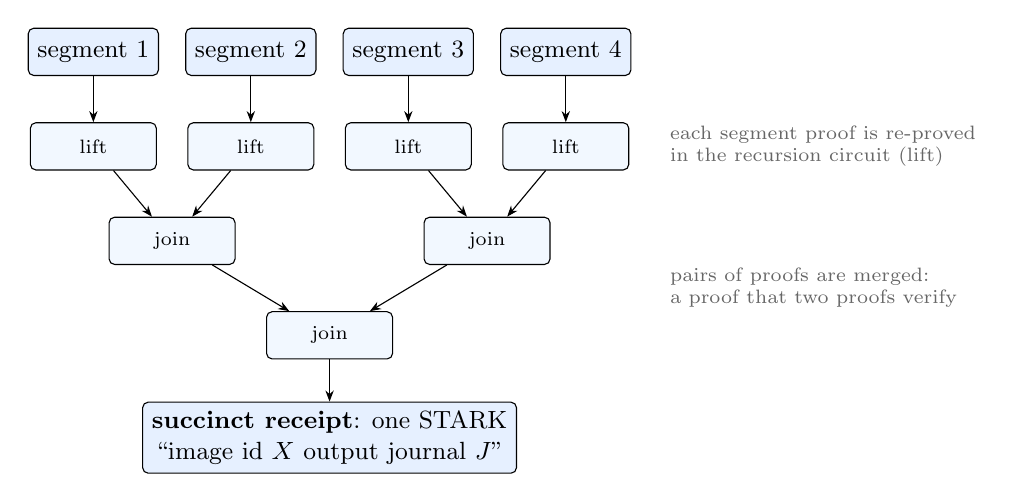
\begin{tikzpicture}[
  font=\small,
  seg/.style={draw, fill=alice, rounded corners=2pt, minimum width=14mm, minimum height=6mm},
  rec/.style={draw, fill=alice!50, rounded corners=2pt, minimum width=16mm, minimum height=6mm, align=center},
  >={Stealth[length=4pt]},
]
\foreach \i/\x in {1/0,2/2,3/4,4/6} { \node[seg] (s\i) at (\x,0) {segment \i}; }
\foreach \i/\x in {1/0,2/2,3/4,4/6} { \node[rec, font=\scriptsize] (l\i) at (\x,-1.2) {lift}; \draw[->] (s\i) -- (l\i); }
\node[rec, font=\scriptsize] (j1) at (1,-2.4) {join};
\node[rec, font=\scriptsize] (j2) at (5,-2.4) {join};
\draw[->] (l1) -- (j1); \draw[->] (l2) -- (j1); \draw[->] (l3) -- (j2); \draw[->] (l4) -- (j2);
\node[rec, font=\scriptsize] (j3) at (3,-3.6) {join};
\draw[->] (j1) -- (j3); \draw[->] (j2) -- (j3);
\node[draw, fill=alice, rounded corners=2pt, align=center, font=\small] (sr) at (3,-4.9) {\textbf{succinct receipt}: one STARK\\``image id $X$ output journal $J$''};
\draw[->] (j3) -- (sr);
\node[font=\scriptsize, text=black!60, align=left, anchor=west] at (7.2,-1.2) {each segment proof is re-proved\\in the recursion circuit (lift)};
\node[font=\scriptsize, text=black!60, align=left, anchor=west] at (7.2,-3) {pairs of proofs are merged:\\a proof that two proofs verify};
\end{tikzpicture}
\caption{Recursion. A long execution is split into segments; each
segment's STARK is lifted into the recursion circuit, and pairs are
joined until one proof remains. Our placeholder guest is a single
segment (3,883 cycles); the Groth16 verifier, if it were the guest,
would be hundreds.}
\label{fig:recursion}
\end{figure}

The result is the \emph{succinct receipt}: one STARK, of fixed size
(about 220~KB), whatever the length of the execution, saying that the
program with image id $X$ ran and output $J$. Every recursion step is
itself a program for the recursion circuit, identified by a
\emph{control id}; the set of allowed recursion programs is committed to
by a Merkle root, the \emph{control root}, which a verifier must know.
The control root is fixed per RISC Zero release, which is why the
version matters later (Section~\ref{sec:verifier}).

\paragraph{Where it runs, and how long.} Anywhere: the proof of concept
proves on the Mac (about 7~s for the placeholder guest, using RISC
Zero's prebuilt prover \texttt{r0vm}) and on an x86 Linux laptop (21~s,
12 cores). The proving time grows with the guest's cycles; a real
withdrawal guest (a signature check and a Merkle path) stays small.

\section{Stage 3: the shrink-wrap into Groth16}
\label{sec:wrap}

The succinct receipt is a STARK of 220~KB whose verification needs many
BabyBear hash computations. To get a small proof with a fixed verifier,
RISC Zero wraps it in Groth16, in two steps.

\begin{figure}[H]
\centering
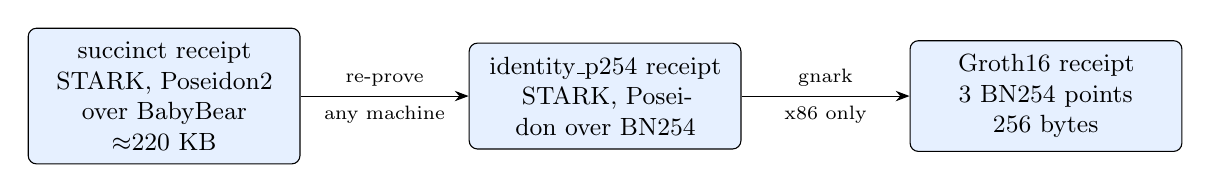
\begin{tikzpicture}[
  font=\small,
  box/.style={draw, rounded corners=3pt, align=center, inner sep=5pt, text width=#1},
  box/.default=31mm,
  >={Stealth[length=5pt]},
]
\node[box, fill=alice] (a) at (0,0) {succinct receipt\\STARK, Poseidon2 over BabyBear\\$\approx$220 KB};
\node[box, fill=alice] (b) at (5.6,0) {identity\_p254 receipt\\STARK, Poseidon over BN254};
\node[box, fill=alice] (c) at (11.2,0) {Groth16 receipt\\3 BN254 points\\256 bytes};
\draw[->] (a) -- node[above, font=\scriptsize] {re-prove} node[below, font=\scriptsize] {any machine} (b);
\draw[->] (b) -- node[above, font=\scriptsize] {gnark} node[below, font=\scriptsize] {x86 only} (c);
\end{tikzpicture}
\caption{The shrink-wrap. The first step changes the hash the STARK is
built with, the second proves ``this STARK verifies'' in a fixed Groth16
circuit.}
\label{fig:wrap}
\end{figure}

\paragraph{Why the proof is re-proved first (identity\_p254).} The
Groth16 circuit is a circuit over BN254's 254-bit field. Inside it,
every BabyBear operation of the STARK's verification would have to be
emulated with non-native arithmetic: far too large. So RISC Zero first
runs one more recursion step, \emph{identity\_p254}, whose job is only
to re-prove the succinct receipt with a STARK whose commitments use a
Poseidon hash over BN254's own field. Verifying \emph{that} STARK inside
the BN254 circuit is affordable. Each step takes the previous step's
output as its input, and each layer exists because the next one could
not take the original directly: arbitrary execution, then one succinct
STARK, then a BN254-friendly STARK, then Groth16.

\paragraph{The Groth16 step.} A fixed circuit verifies an identity\_p254
STARK and outputs a Groth16 proof: three points on the BN254 curve, $A$
and $C$ on the group $G_1$ (64 bytes each, two 32-byte coordinates) and
$B$ on $G_2$ (128 bytes), 256 bytes in all. Its \emph{public inputs},
the values a verifier must supply, are:
\begin{itemize}[leftmargin=1.5em]
\item the control root (Section~\ref{sec:stark}), as two 128-bit halves:
  which recursion programs were allowed;
\item the \emph{claim digest}, as two halves: a hash of the image id,
  the journal and the exit status;
\item the BN254 control id: which identity\_p254 program was used.
\end{itemize}
The verifier recomputes the claim digest itself from the image id and
the journal it is given, so the proof is bound to exactly that program
and that output.

\paragraph{Where it runs, and how long.} RISC Zero runs the Groth16
prover (gnark, with its proving key) in a Docker image built for x86
only. This is the one step that needs an x86 machine. On the 12-core
Linux laptop, the whole wrap took 102~s; it needs several gigabytes of
memory (it was killed at under 2~GB on the Mac's small Docker VM).

\section{Stage 4: the input to the BitVMX verifier}
\label{sec:input}

BitVMX's Groth16 verifier takes its input as a flat byte string.
Points are stored compressed: only the $x$ coordinate and a sign bit,
since $y$ can be recomputed from the curve equation. That makes $A$ and
$C$ 32 bytes and $B$ 64:

\begin{figure}[H]
\centering
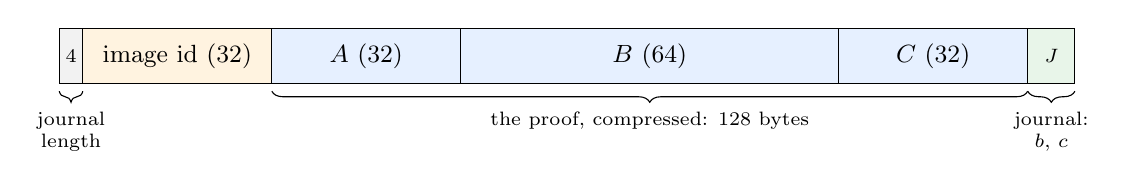
\begin{tikzpicture}[font=\small, x=0.075cm]
\def\h{0.7}
\draw[fill=black!5] (0,0) rectangle (4,\h); \node at (2,\h/2) {\scriptsize 4};
\draw[fill=fixed] (4,0) rectangle (36,\h); \node at (20,\h/2) {image id (32)};
\draw[fill=alice] (36,0) rectangle (68,\h); \node at (52,\h/2) {$A$ (32)};
\draw[fill=alice] (68,0) rectangle (132,\h); \node at (100,\h/2) {$B$ (64)};
\draw[fill=alice] (132,0) rectangle (164,\h); \node at (148,\h/2) {$C$ (32)};
\draw[fill=chain] (164,0) rectangle (172,\h); \node at (168,\h/2) {\scriptsize $J$};
\draw[decorate, decoration={brace, amplitude=4pt, mirror}] (0,-0.1) -- (4,-0.1) node[midway, below=4pt, font=\scriptsize, align=center] {journal\\length};
\draw[decorate, decoration={brace, amplitude=4pt, mirror}] (36,-0.1) -- (164,-0.1) node[midway, below=4pt, font=\scriptsize] {the proof, compressed: 128 bytes};
\draw[decorate, decoration={brace, amplitude=4pt, mirror}] (164,-0.1) -- (172,-0.1) node[midway, below=4pt, font=\scriptsize, align=center] {journal:\\$b$, $c$};
\end{tikzpicture}
\caption{The verifier's 172-byte input for our guest. The journal length
is counted in 4-byte words (here 2). The sample proof used before had a
4-byte journal and so 168 bytes.}
\label{fig:input}
\end{figure}

Because the journal is part of the input, $b$ and $c$ sit at fixed byte
offsets, and so in fixed 4-byte input words. That is what lets the
Bitcoin contract read them later: Alice signs every input word with a
one-time key when the dispute starts, and the contract's payout scripts
read the bits of $b$ from her signature on that word.

\section{Stage 5: the verifier program}
\label{sec:verifier}

The verifier is a C program (FairgateLabs' \texttt{bitvmx-zk-verifier})
compiled to RISC-V for BitVMX's emulator. It is fixed: the same binary
checks every withdrawal. Its constants are baked in: the Groth16
verifying key of RISC Zero's circuit, the control root and the BN254
control id. Given the 172 bytes, it
\begin{enumerate}[leftmargin=1.5em]
\item decompresses the three points;
\item recomputes the claim digest from the image id and the journal;
\item computes the linear combination of verifying-key points weighted
  by the public inputs;
\item checks the pairing equation
  $e(A,B) = e(\alpha,\beta)\cdot e(L,\gamma)\cdot e(C,\delta)$,
  where $\alpha,\beta,\gamma,\delta$ come from the verifying key and $L$
  is the combination of step 3;
\item halts with exit code 0 if it holds, otherwise non-zero.
\end{enumerate}
Pairings on a 32-bit machine without big-number instructions are slow:
the run on our receipt took \textbf{477,641,148 steps} (57~s in the
emulator on the Mac) and halted with exit code~0. With the journal's $b$
changed from 9 to 10 it halted with exit code~1: the proof is bound to
the journal.

\paragraph{Why versions matter.} The baked constants belong to one RISC
Zero release family. The proof of concept found that the shipped
verifier carries RISC Zero 3.0's control root (\texttt{a54dc85a\ldots}),
so receipts made with RISC Zero 3.0.x verify with it unchanged; an
earlier sample proof, made with older parameters, needed the constants
patched in the binary. The proving tools are therefore pinned to RISC
Zero 3.0.6.

\section{Stage 6: bisecting the verifier's execution}
\label{sec:bisection}

Suppose Alice claims ``the verifier, run on these 172 bytes, halts with
exit code 0'' and the hub disagrees. Both can run the verifier locally
(57~s), and both are bound to the same input, since Alice has signed it.
Instead of asking Bitcoin to run 478 million steps, they search for the
first step on which they disagree.

\paragraph{State hashes.} BitVMX summarises the machine after step $i$
by a hash $h_i$, chained so that $h_i$ depends on $h_{i-1}$ and on what
step $i$ did (the instruction, the values it read and wrote, the next
program counter). Agreeing on $h_i$ means agreeing on the whole
execution up to step $i$.

\paragraph{The search.} Alice (the prover) and the hub (the verifier)
both know $h_0$ (the program's start) and disagree about the end. In
each round Alice publishes the hash at the midpoint of the current
interval; the hub compares it with its own and picks the half in which
they disagree. After $\log_2$ of the number of steps rounds, the
interval is a single step $k \to k+1$: they agree on $h_k$ and disagree
on $h_{k+1}$.

\begin{figure}[H]
\centering
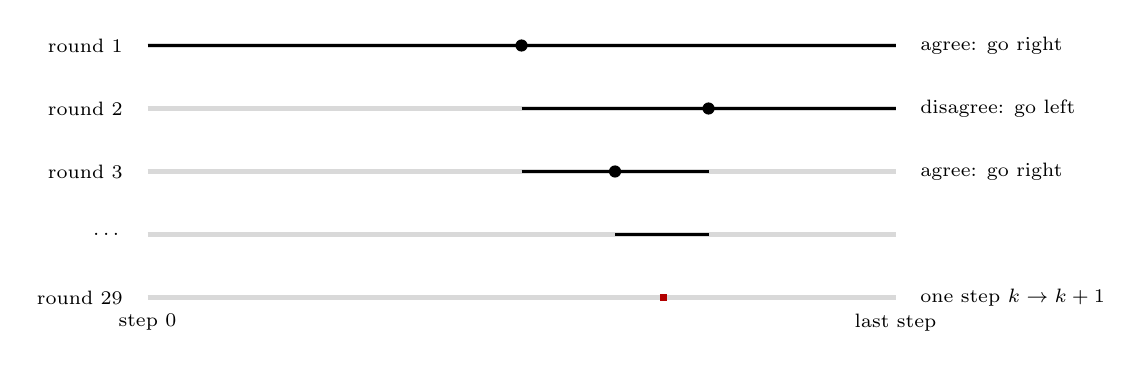
\begin{tikzpicture}[font=\small, x=0.95cm, y=0.8cm]
\tikzset{row/.style={font=\scriptsize, anchor=east}, ann/.style={font=\scriptsize, anchor=west}}
% the whole execution, faint, on every row
\foreach \y in {0,-1,-2,-3,-4} { \draw[black!15, line width=2pt] (0,\y) -- (10,\y); }
\node[font=\scriptsize, below] at (0,-4.1) {step 0};
\node[font=\scriptsize, below] at (10,-4.1) {last step};
% round 1
\node[row] at (-0.2,0) {round 1};
\draw[thick] (0,0) -- (10,0); \fill (5,0) circle (2.2pt);
\node[ann] at (10.2,0) {agree: go right};
% round 2
\node[row] at (-0.2,-1) {round 2};
\draw[thick] (5,-1) -- (10,-1); \fill (7.5,-1) circle (2.2pt);
\node[ann] at (10.2,-1) {disagree: go left};
% round 3
\node[row] at (-0.2,-2) {round 3};
\draw[thick] (5,-2) -- (7.5,-2); \fill (6.25,-2) circle (2.2pt);
\node[ann] at (10.2,-2) {agree: go right};
% dots
\node[row] at (-0.2,-3) {\ldots};
\draw[thick] (6.25,-3) -- (7.5,-3);
% final
\node[row] at (-0.2,-4) {round 29};
\draw[line width=2.5pt, red!70!black] (6.85,-4) -- (6.95,-4);
\node[ann] at (10.2,-4) {one step $k \to k+1$};
\end{tikzpicture}
\caption{Binary search over the verifier's execution. In each round the
hub compares Alice's midpoint hash with its own and keeps the half in
which they disagree; at the end they agree on $h_k$ but not on
$h_{k+1}$. For the Groth16 verifier,
29 rounds narrow $2^{29}$ steps to one.}
\label{fig:bisection}
\end{figure}

\paragraph{The last step.} Now Bitcoin has to judge one RISC-V
instruction: given the state committed by $h_k$, does executing step
$k+1$ produce $h_{k+1}$? Alice reveals the step's details (the
instruction, the registers and memory it read, what it wrote) and a
script checks that they hash to the agreed $h_k$, that the instruction
computes what it claims, and that the result hashes to her $h_{k+1}$. If
the hub suspects a value she claims to have read, a second, shorter
search (the \emph{read challenge}) finds the step that last wrote that
address. In the proof of concept the final step of the verifier, its
halting system call, is proved in a 58.5~kvB transaction; the
disputed step is a single instruction, so the cost does not depend on
the program.

\paragraph{Honesty is enough.} An honest Alice can always answer, because
her hashes come from the true execution; an honest hub can always find a
disagreement with a false claim, because the true execution ends
differently. Whoever is wrong runs out of moves.

\section{Where LN-GAP comes in}
\label{sec:lngap}

BitVMX plays the search on Bitcoin: every round is a transaction with a
timeout. LN-GAP 2.5 plays it instead as a game inside the channel. Each
move (a midpoint, a choice) is a signed message between Alice and the
hub, so a withdrawal dispute between honest parties costs nothing on
chain until its last step. What the game needs from outside is a record
of \emph{when} each move was made, so that a party who stops answering
can be told apart from one whose answer was suppressed. That record is
kept by a venue of bonded members, who put Merkle roots of the moves
they received on Bitcoin in their periodic seal closings; a party
claiming its opponent stalled is answered by a rebuttal that proves the
move was dated in time. Only when someone misbehaves (stalls, makes a
false claim, or a member fails) does the game continue on chain, one
move per transaction, at the cost of the bond of whoever forced it.
LN-GAP 2.5 itself is not published; its successor,
Lichen~(\url{https://github.com/AdamISZ/lichen}), drops the venue and
plays the search on Bitcoin, as BitVMX does. For the proving pipeline,
what matters is that the program being searched is always the Groth16
verifier of Section~\ref{sec:verifier}.

\begin{figure}[H]
\centering
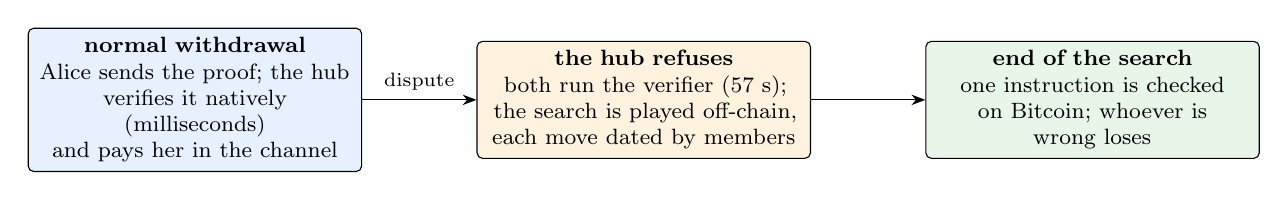
\begin{tikzpicture}[font=\footnotesize, >={Stealth[length=5pt]}, y=0.9cm]
\node[draw, rounded corners=2pt, fill=alice, align=center, text width=40mm] (n) at (0,0) {\textbf{normal withdrawal}\\Alice sends the proof; the hub\\verifies it natively (milliseconds)\\and pays her in the channel};
\node[draw, rounded corners=2pt, fill=fixed, align=center, text width=40mm] (d) at (5.7,0) {\textbf{the hub refuses}\\both run the verifier (57 s);\\the search is played off-chain,\\each move dated by members};
\node[draw, rounded corners=2pt, fill=chain, align=center, text width=40mm] (c) at (11.4,0) {\textbf{end of the search}\\one instruction is checked\\on Bitcoin; whoever is\\wrong loses};
\draw[->] (n) -- node[above, font=\scriptsize] {dispute} (d);
\draw[->] (d) -- (c);
\end{tikzpicture}
\caption{Most withdrawals stop at the first box. The search is played
only when the hub disputes, and reaches Bitcoin only at its end.}
\end{figure}

\section{Who does what, where, and how long}
\label{sec:who}

\begin{center}
\small
\begin{tabularx}{\linewidth}{@{}>{\raggedright\arraybackslash}p{40mm}>{\raggedright\arraybackslash}p{30mm}>{\raggedright\arraybackslash}p{28mm}L@{}}
\toprule
step & who & where & measured \\
\midrule
compile the guest & both (to agree on the image id) & any machine & seconds \\
prove (STARK) & Alice & any machine & 7 s (Mac), 21 s (x86, 12 cores) \\
wrap (identity\_p254 + Groth16) & Alice & x86 for the Groth16 step & 102 s (x86, 12 cores); several GB \\
verify natively & the hub & any machine & milliseconds \\
run the BitVMX verifier & both, only in a dispute & any machine & 478M steps, 57 s \\
the search & both, only in a dispute & off-chain, in the channel & 29 rounds (59 moves) \\
the last step & Alice proves it, or the hub's challenge stands & Bitcoin & 58.5 kvB \\
\bottomrule
\end{tabularx}
\end{center}

\section{Practical notes from the proof of concept}
\label{sec:practical}

\begin{itemize}[leftmargin=1.5em]
\item \emph{Pin the RISC Zero version} to the release whose constants
  the verifier binary carries (3.0.x for the shipped binary). The image
  id depends on the toolchain too.
\item \emph{The Groth16 step needs x86 and Docker.} On Apple silicon,
  RISC Zero's in-process prover also needs Xcode's Metal compiler; using
  the prebuilt \texttt{r0vm} through RISC Zero's client API avoids it.
\item \emph{Snap-installed Docker} cannot see \texttt{/tmp}, where RISC
  Zero hands the Groth16 step its files; set \texttt{RISC0\_WORK\_DIR}
  to a directory under your home.
\item \emph{Memory:} the Groth16 step was killed on a 2~GB VM and ran on
  a 38~GB laptop; budget 16~GB.
\item \emph{Encoding:} the verifier wants compressed points and the
  journal length in words; FairgateLabs' \texttt{proof-as-input} tool
  produces the layout of Figure~\ref{fig:input}.
\end{itemize}

\section*{Glossary}
\addcontentsline{toc}{section}{Glossary}

\begin{description}[leftmargin=1.5em, style=nextline]
\item[BabyBear] the 31-bit prime field $15\cdot 2^{27}+1$ RISC Zero's
  STARKs compute in.
\item[BN254] a pairing-friendly elliptic curve (also called alt\_bn128);
  Groth16 proofs here live on it.
\item[BitVMX] a protocol and RISC-V emulator for disputing a program's
  execution on Bitcoin by bisection, by FairgateLabs.
\item[claim digest] a hash of the image id, the journal and the exit
  status: what a RISC Zero proof is ultimately about.
\item[control id, control root] identifiers of RISC Zero's recursion
  programs, and the Merkle root of the allowed ones; fixed per release.
\item[gnark] a Go library for SNARKs; RISC Zero uses it for the Groth16
  step.
\item[Groth16] a pairing-based SNARK with constant-size proofs (three
  curve points) and a per-circuit trusted setup.
\item[guest] the program whose execution is proved, run in RISC Zero's
  zkVM.
\item[identity\_p254] the recursion step that re-proves a STARK with a
  BN254-friendly hash, so that Groth16 can verify it.
\item[image id] the hash of a guest's compiled memory image.
\item[journal] the guest's public output.
\item[receipt] RISC Zero's proof object (a journal plus a seal): segment,
  succinct, or Groth16.
\item[recursion] proving the verification of proofs, to fold many into
  one.
\item[segment] a slice of a long execution, proved separately.
\item[shrink-wrap] the conversion of a succinct receipt into a Groth16
  receipt.
\item[STARK] a hash-based proof system with a transparent setup and
  larger proofs.
\item[witness] the private input that makes a statement true.
\item[zkVM] a virtual machine whose executions can be proved.
\end{description}

\end{document}
